\section{实验}
\label{sec:experiments}

\subsection{实验设置与评价协议}
主实验采用 Cityscapes~\cite{cordts2016cityscapes} $\rightarrow$ DensePASS~\cite{ma2021densepass}：Cityscapes 为有标注源域，DensePASS 为无标签目标域，并使用其验证集评估从透视街景到全景街景的适配。模型为 OmniSAM~\cite{zhong2025omnisam} / sam2\_s~\cite{ravi2025sam2}，采用 13 类协议；所有主结果均来自单随机种子 full protocol，未包含跨数据集或多随机种子结论。源域标签用于监督分割损失，目标域训练阶段不使用人工标签；DensePASS 验证标签只用于模型评估。Baseline 与 Ours 采用相同数据列表、预处理和验证流程，区别仅在训练阶段是否启用 MTC 与 SMR。

本文以 mIoU 衡量类别级分割质量，并报告 mAcc、PixAcc、FWIoU 与 mDice；BFScore 补充衡量边界一致性。mIoU 反映各类别区域重叠的平均水平，BFScore 对 ERP 接缝、细长结构和局部边界误差更敏感，二者共同刻画 token 约简的质量代价。效率指标包括训练耗时与 Iter 时间。Memory Attention Time 和 Memory Tokens 仅用于固定伪标签消融设置，不能与端到端训练时间混用。

\subsection{实现细节}
MTC 与 SMR 置于 memory attention 前，分别改变记忆的空间密度和检索子集，不修改源域监督、目标域伪标签损失或分割输出。主结果比较 OmniSAM 与 Ours (MTC+SMR)。后者在训练阶段同时使用辅助置信掩码，但论文主名称突出直接改变 memory 计算的 MTC 与 SMR；伪标签生成阶段保持原流程，以避免将训练效率收益与伪标签变化混合解释。PQR 独立作为伪标签可靠性辅助消融。

\subsection{主结果}
\begin{table}[t]
  \centering
  \small
  \setlength{\tabcolsep}{4pt}
  \renewcommand{\arraystretch}{1.08}
  \caption{Cityscapes $\rightarrow$ DensePASS full protocol 下的分割性能与训练效率比较。所有结果采用 \texttt{sam2\_s}、13 类协议和单随机种子设置；BFScore 来自同一验证流程的 \texttt{[ValSummary]}。}
  \label{tab:main_results}
  \begin{tabular}{lccccc}
    \toprule
    方法 & mIoU$\uparrow$ & BFScore$\uparrow$ & 训练耗时$\downarrow$ & Iter 时间$\downarrow$ & 降幅 \\
    \midrule
    OmniSAM & \textbf{60.26} & \textbf{39.97} & 43m53s & 5.27s & -- \\
    Ours (MTC+SMR) & 60.16 & 39.86 & \textbf{34m03s} & \textbf{4.09s} & \textbf{22.4\%} \\
    \bottomrule
  \end{tabular}
\end{table}


表~\ref{tab:main_results} 显示，Ours (MTC+SMR) 的 mIoU 和 BFScore 分别比 OmniSAM 低 0.10 和 0.11。轻微的精度与边界代价说明 token 约简并非无损，但主要分割质量保持稳定，支持历史记忆中存在可压缩冗余。区域指标和边界指标的变化幅度接近，未出现大范围预测失效；由于采用单随机种子，这些差异仍应视为该协议下的观察。

\subsection{效率分析}
表~\ref{tab:main_results} 同时给出端到端训练效率：Ours (MTC+SMR) 的训练耗时与 Iter 时间均下降约 22.4\%。该收益来自进入 memory attention 的 token 规模降低。端到端时间同时包含 memory 之外的计算，因此其下降幅度小于纯 attention 模块可能达到的比例，但更能反映完整 UDA 训练的实际成本。该结果仅说明训练阶段效率；本文未验证推理加速或显存下降。

\subsection{定性结果}
图~\ref{fig:qualitative_full_protocol} 比较了 OmniSAM baseline 与 MTC+SMR。两者保持相近的主要场景结构，局部边界和小目标仍有差异，与 BFScore 的轻微下降一致；这些样例仅作定性观察。

\begin{figure}[t]
    \centering
    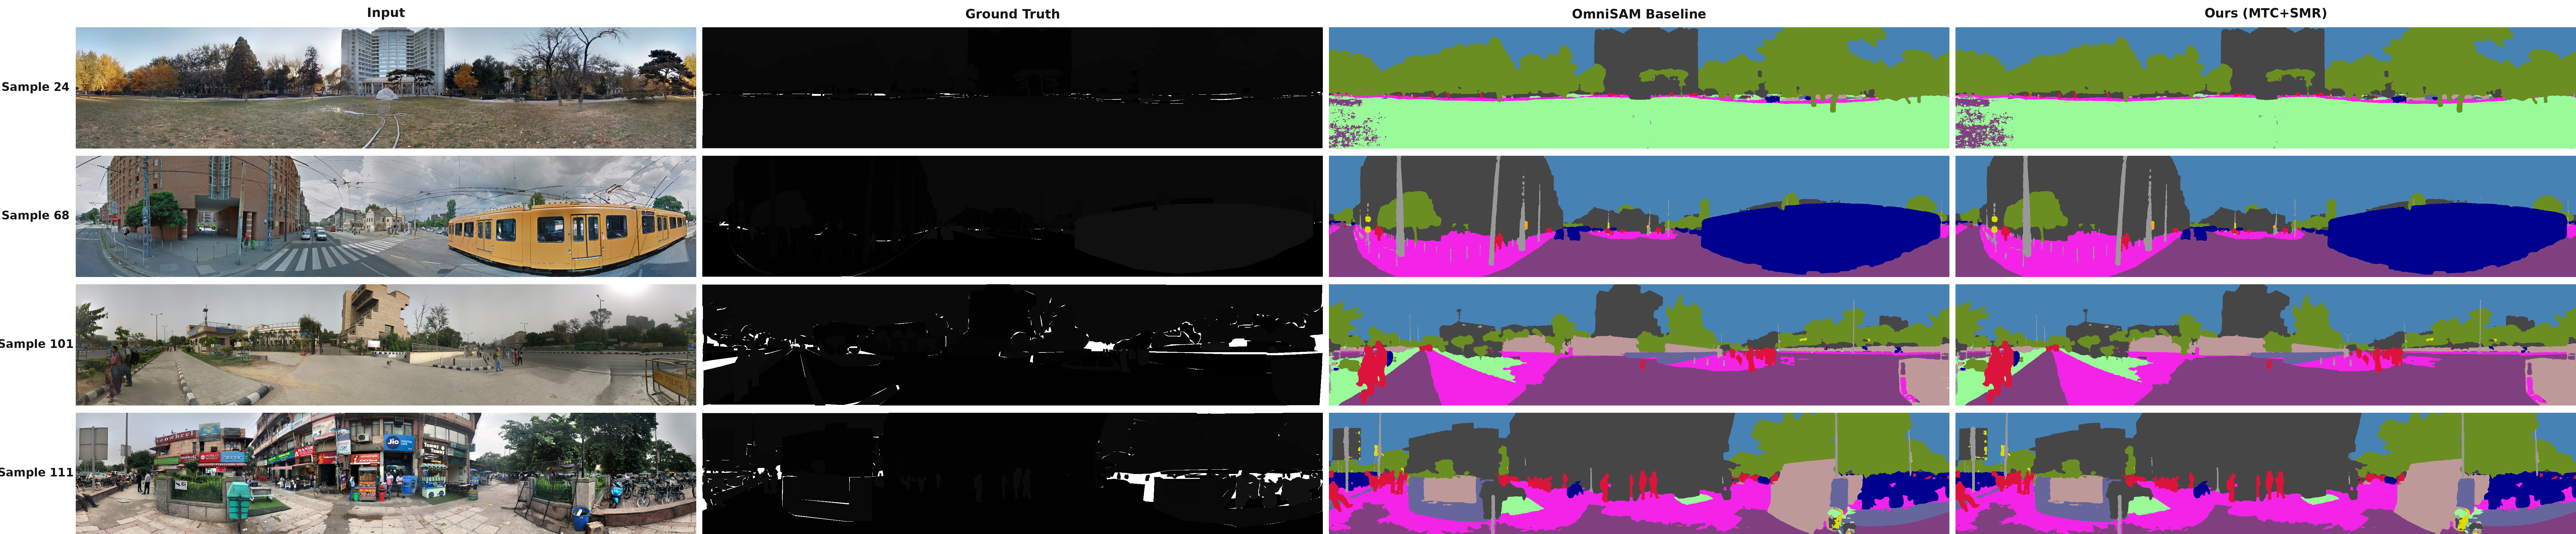
\includegraphics[width=\linewidth]{figures/fig_qualitative_full_protocol.png}
    \caption{Cityscapes $\rightarrow$ DensePASS full protocol 下的定性分割结果。各行依次展示目标域输入、真实标注、OmniSAM baseline 和本文 MTC+SMR 配置的预测。Baseline 与 Ours 使用相同的 sam2\_s、13 类协议、数据预处理和 ERP 推理流程。}
    \label{fig:qualitative_full_protocol}
\end{figure}
